\chapter{Evaluation}
\label{results}

The aim of this chapter is to critically analyse the usefulness and accuracy of the developed extractor. Using a Simulink model, a Markov Decision Process is extracted and then the responses of both systems to two different stimulation signals are compared. This chapter serves as an evaluation of the approach developed for this thesis.

\section{Setup}

In the following, the evaluation experiment setup is described. The test model, the stimulation signals and the model's Simulink implementation are introduced.

\subsection{Test Model}

The model used for this result analysis is a third-order Butterworth filter, chosen mainly because of it's interesting overshoot properties. The filter is modeled using the transfer function \cite{ccs}

\[
H(s) = \frac{1}{s^3+2s^2+2s+1}.
\]

Section~\ref{eval_sim_models} presents the Simulink implementation of this filter.

\subsection{Stimulation Signals}

For each experiment a different signal was used. Firstly a constant input signal and secondly a scaled step signal. These two  signals $u_1(t)$ and $u_2(t)$ are defined as:
\begin{align}
u_1(t) &= 0.6667, \nonumber \\
u_2(t) &= \left\{
            \begin{array}{l l}
                0.6667, & \quad t < 10\\
                4, & \quad t \geq 10 \\
            \end{array}.\nonumber \right
\end{align}


\begin{figure}
\begin{center}
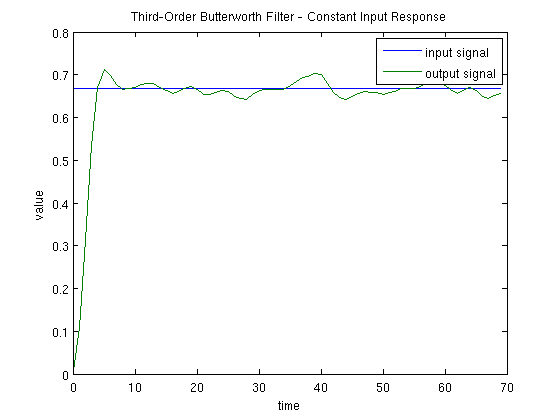
\includegraphics[height=9cm]{media/bw/bw_const_response}\\
\end{center}
\caption{Response of Butterworth-Filter system to constant input}
\label{bw_const_response}
\end{figure}

\begin{figure}
\begin{center}
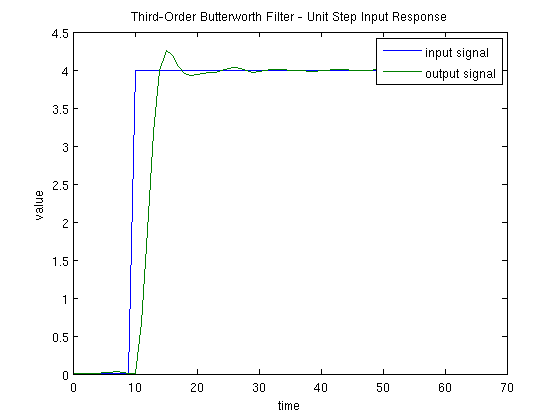
\includegraphics[height=9cm]{media/bw/bw_step_response}\\
\end{center}
\caption{Response of Butterworth-Filter system to a scaled step input (step at t=10)}
\label{bw_step_response}
\end{figure}

Figures~\ref{bw_const_response} and~\ref{bw_step_response} show the standard response of the filter to these inputs, as well as the input signals themselves. Note that even though $u_1(t)$ is defined here as a constant signal, it is in fact a step signal, with step time $t=0$ and step value $0.6667$. This effect occurs because there is no way to let the Simulink model start with a past signal value. Nonetheless it will be referred to here as the constant signal, because of the relatively small difference between the initial state and the step.

\subsection{Simulink Models}
\label{eval_sim_models}

The filter was implemented three different times as a Simulink model, once for each input signal and once for the extraction. Figures~\ref{bw_const_mdl} and~\ref{bw_step_mdl} show the model for input signals $u_1(t)$ and $u_2(t)$, respectively. Figure~\ref{bw_extract_mdl} shows the model as it was prepared for the extraction (with root level inputs and outputs).

\begin{figure}
\begin{center}
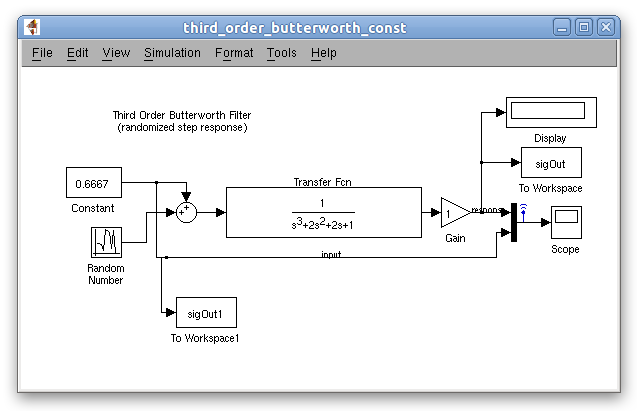
\includegraphics[height=9cm]{media/bw/bw_const_mdl}\\
\end{center}
\caption{Implementation of a Butterworth-Filter in Simulink with a constant input}
\label{bw_const_mdl}
\end{figure}

\begin{figure}
\begin{center}
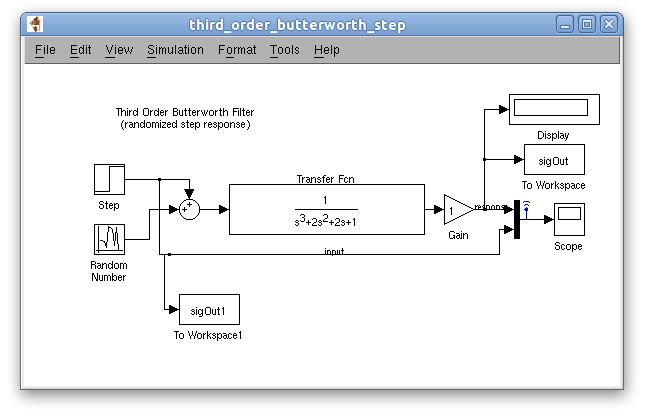
\includegraphics[height=9cm]{media/bw/bw_step_mdl}\\
\end{center}
\caption{Implementation of a Butterworth-Filter in Simulink with a scaled step input (step at t=10) MUST FIX FOR 0 BOUND!!}
\label{bw_step_mdl}
\end{figure}

\begin{figure}
\begin{center}
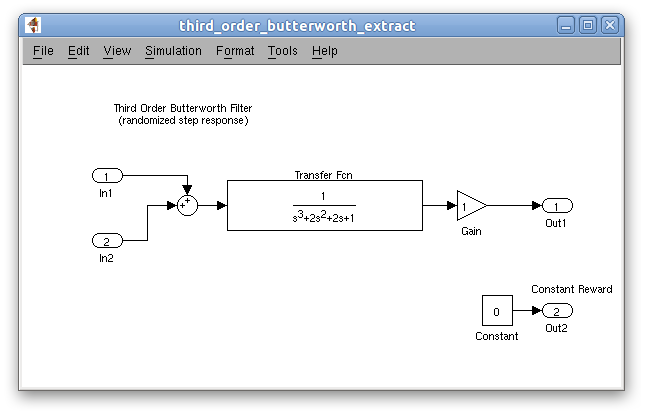
\includegraphics[height=9cm]{media/bw/bw_extract_mdl}\\
\end{center}
\caption{Butterworth-Filter Simulink model prepared for MDP extraction}
\label{bw_extract_mdl}
\end{figure}

\section{Result}
\label{sec:resultsextraction}

In order to evaluate the usefulness of the extraction approach presented in this thesis, the test model was transformed into a Markov Decision Process. As described in section~\ref{subsec:extractconf}, a number of choices must be made. The configuration of this extraction is relatively simple because of the model's simplicity (single input, single output). The following parameters defined the extraction:

\begin{itemize}
\item input: $u$, $u_{min} = 0$, $u_{max} = 6$
\item input granularity: $N_{u}=10$
\item random input: normally distributed with mean $\mu=0$ and variance $\sigma^2 = 0.001$
\item output boundaries: $y_{min}=0$, $y_{max}=10$
\item output discretization: $n_1=-2$
\item probabilistic simulation, number of runs: $n_{psim}$ = 20
\end{itemize}

The extraction took approximately 40 hours on a dual-core HP workstation with 2 GB of RAM. 634 states were discovered during the extraction, meaning that the transition probability matrix is of dimension $636\times636\times10$ (the two extra states are the \textit{out-of-bound state} and the \textit{error state} discussed in sections~\ref{subsec:outputboundaries} and~\ref{subsec:simerrors}). The next section presents the extractor's evaluation.

\section{Evaluation}

Two validation comparisons were made, comparing the response of the Simulink model and the response of the Markov Decision Process to both the stimulation signal $u_1(t)$ and $u_2(t)$. The `compare' function ran 100 simulation of both the pre-configured Simulink models and the Markov Decision Process. The resulting plots and a short analysis thereof can be found the next two sections.

\subsection{Response to Constant Signal}
\label{sec:respconst}

\begin{figure}
\begin{center}
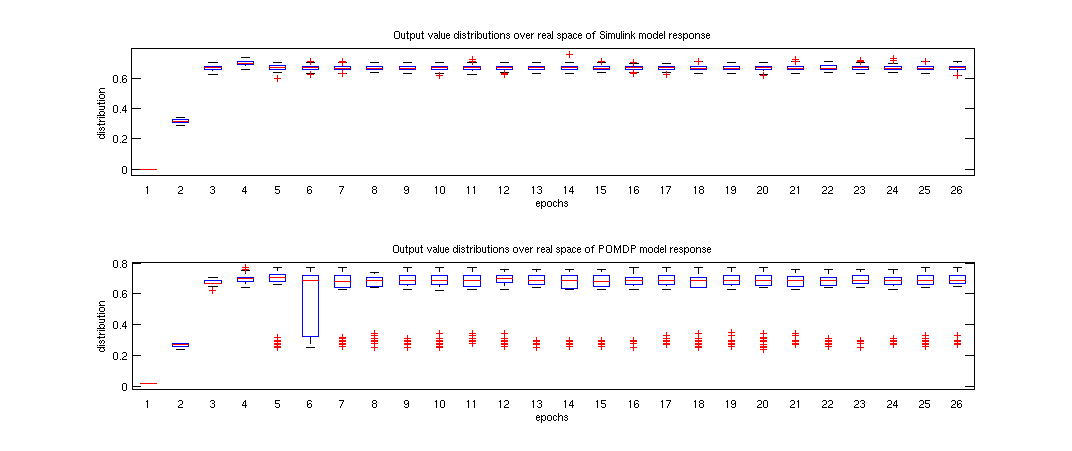
\includegraphics[width=18cm]{media/bw/bw_val_const_real_box}\\
\end{center}
\caption{Box plots of output value distributions of Simulink and MDP responses to signal $u_1(t)$}
\label{bw_val_const_real_box}
\end{figure}

\begin{figure}
\begin{center}
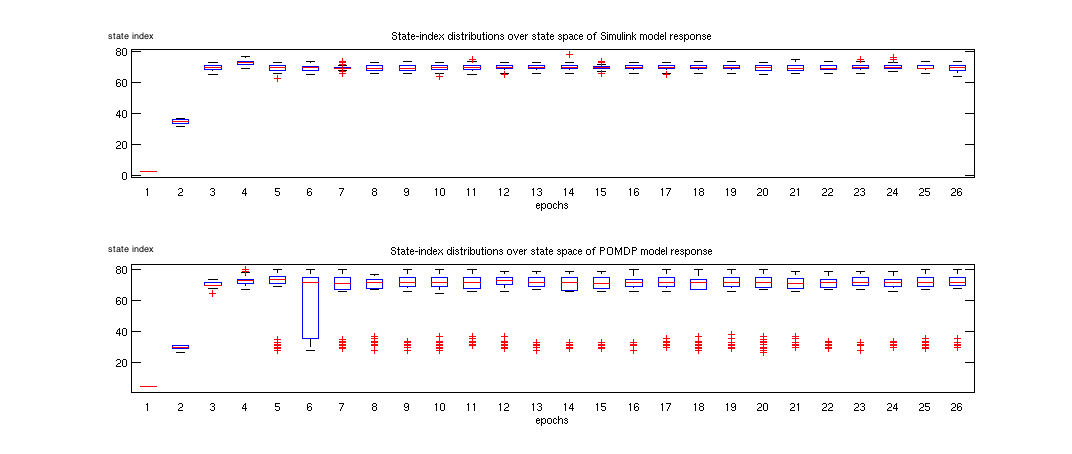
\includegraphics[width=18cm]{media/bw/bw_val_const_state_box}\\
\end{center}
\caption{Box plots of state-index distributions of Simulink and MDP responses to signal $u_1(t)$}
\label{bw_val_const_state_box}
\end{figure}

\begin{figure}
\begin{center}
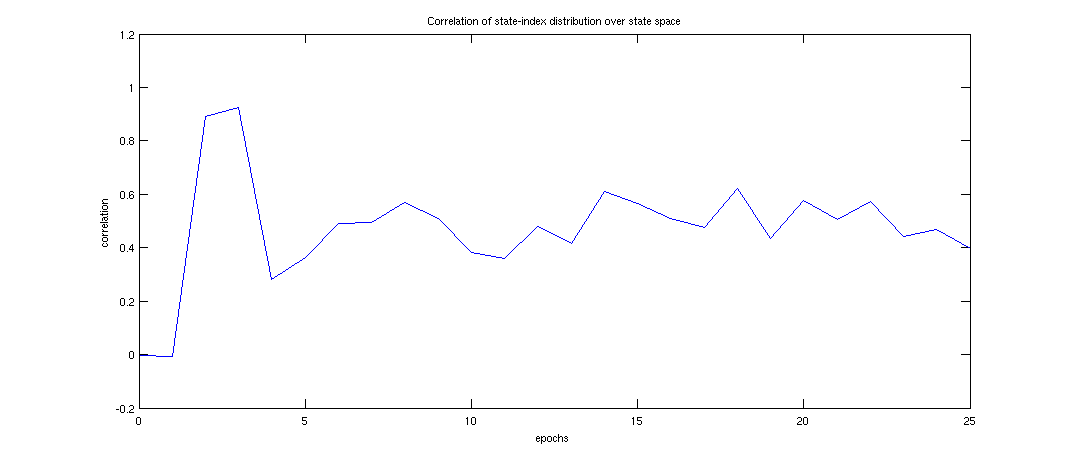
\includegraphics[width=18cm]{media/bw/bw_val_const_state_corr}\\
\end{center}
\caption{Plot of state-index distributions correlation of the Simulink and MDP responses to signal $u_1(t)$}
\label{bw_val_const_state_corr}
\end{figure}

\begin{figure}
\begin{center}
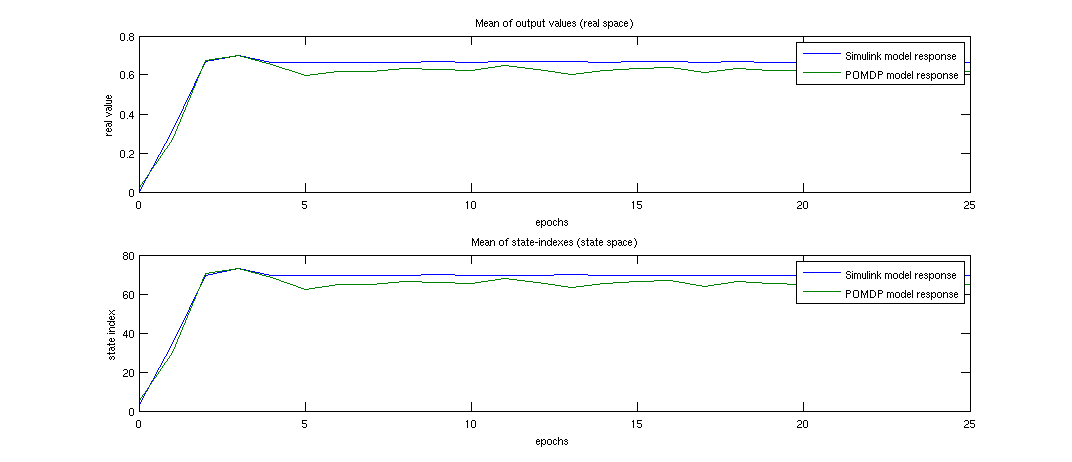
\includegraphics[width=18cm]{media/bw/bw_val_const_real_mean}\\
\end{center}
\caption{Plot of the real output value mean of Simulink and MDP responses to signal $u_1(t)$}
\label{bw_val_const_real_mean}
\end{figure}

In this section, the response differences between the Simulink and the MDP model will be discussed.

Figures~\ref{bw_val_const_real_box} and~\ref{bw_val_const_state_box} show the response distributions in both the real number space and the state space. Note that, as described in section~\ref{subsec:validationmethodology}, the conversion of the Simulink model's scalar output values to the Markov Process's state space provides an analytical base for evaluating the effect of the discretization (see section~\ref{subsec:outputdiscretization}) on the extracted system's behaviour. In this case it is immediately obvious, that the discretization does not have a strong influence on the accuracy of the response, as the Simulink responses look almost exactly similar in both the real space and the state space and the MDP's responses also look equally distributed in both spaces. These box plots do however show that the MDP's responses are distributed with a much higher variance than those of the Simulink model. Additionaly two suprising patterns can be observed. Firstly the MDP system behaves differently at epoch six, where the response variance is much higher than for the the other epochs, and secondly, the MDP's responses have a number of ouliers that remain at much lower values, both in real and in state space.

The correlation plot in figure~\ref{bw_val_const_state_corr} also offers interesting insights. The average correlation between state distributions averages at around 0.4. This value is quite low and probably caused by the combination of a large number of states and the rather large variance discussed in the previous paragraph. Interestingly the correlation jumps to much higher values at epochs two and three. This seems to indicate that whilst the correlation is quite low at steady state, it increases when the system radically changes.

Finally, figure~\ref{bw_val_const_real_mean} shows the means of all responses in both state and real space. The plots show a strong correlation of the mean values. This is valuable information because it shows that even though the MDP's responses vary greatly, they do in fact, in average, produce a very similar response to the original model's. The different outputs, both in real and in state space, at steady state should also be noted and will be discussed in chapter~\ref{discussion}.

\subsection{Response to Step Signal}
\label{sec:respstep}

\begin{figure}[h!]
\begin{center}
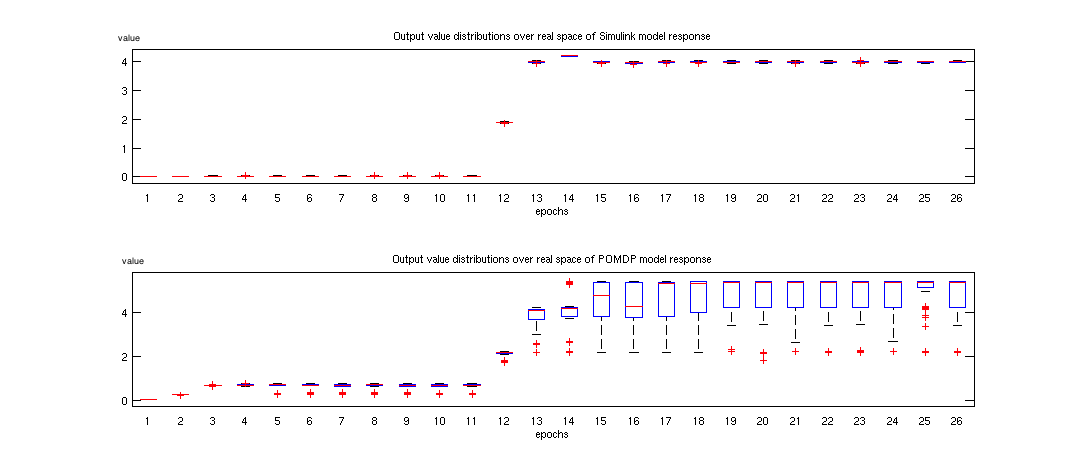
\includegraphics[width=18cm]{media/bw/bw_val_step_real_box}\\
\end{center}
\caption{Box plots of output value distributions of Simulink and MDP responses to signal $u_2(t)$}
\label{bw_val_step_real_box}
\end{figure}

\begin{figure}[h!]
\begin{center}
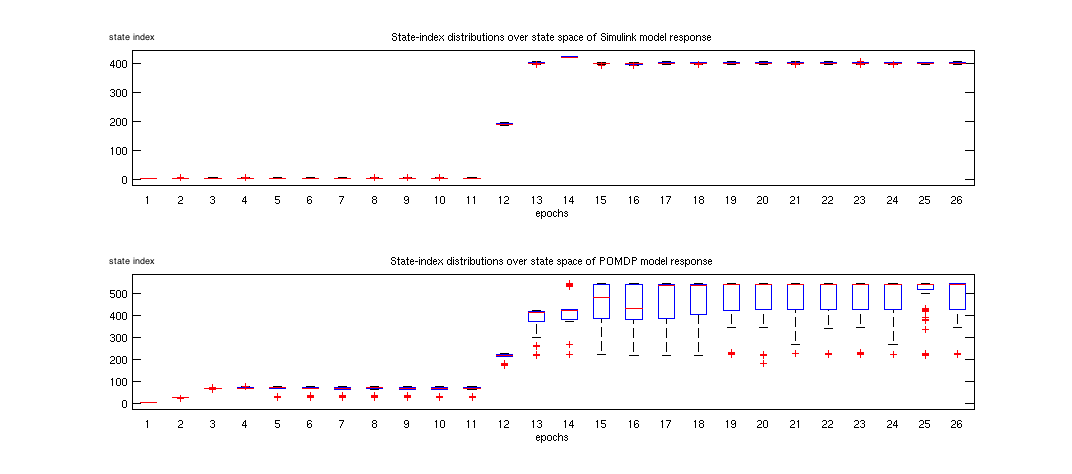
\includegraphics[width=18cm]{media/bw/bw_val_step_state_box}\\
\end{center}
\caption{Box plots of state-index distributions of Simulink and MDP responses to signal $u_2(t)$}
\label{bw_val_step_state_box}
\end{figure}

\begin{figure}[h!]
\begin{center}
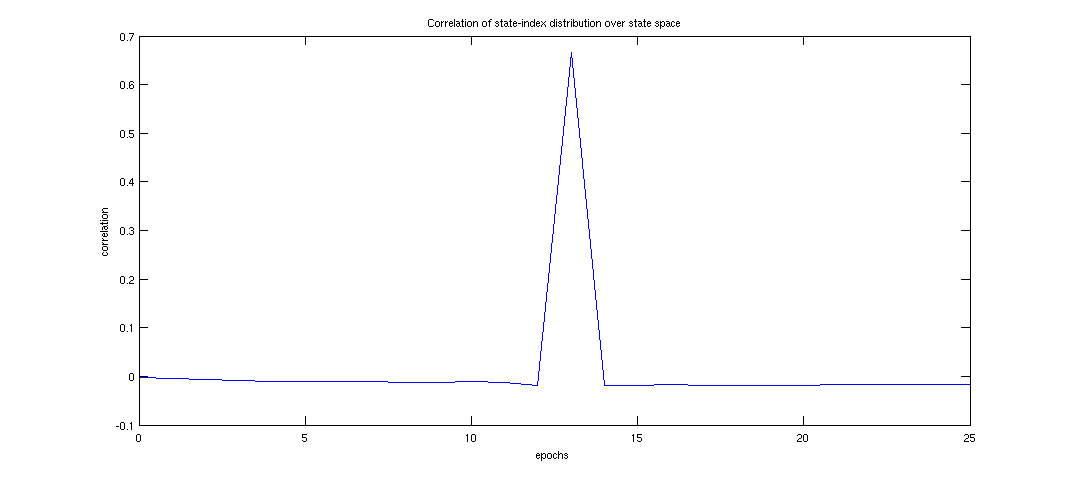
\includegraphics[width=18cm]{media/bw/bw_val_step_state_corr}\\
\end{center}
\caption{Plot of state-index distributions correlation of the Simulink and MDP responses to signal $u_2(t)$}
\label{bw_val_step_state_corr}
\end{figure}

\begin{figure}[h!]
\begin{center}
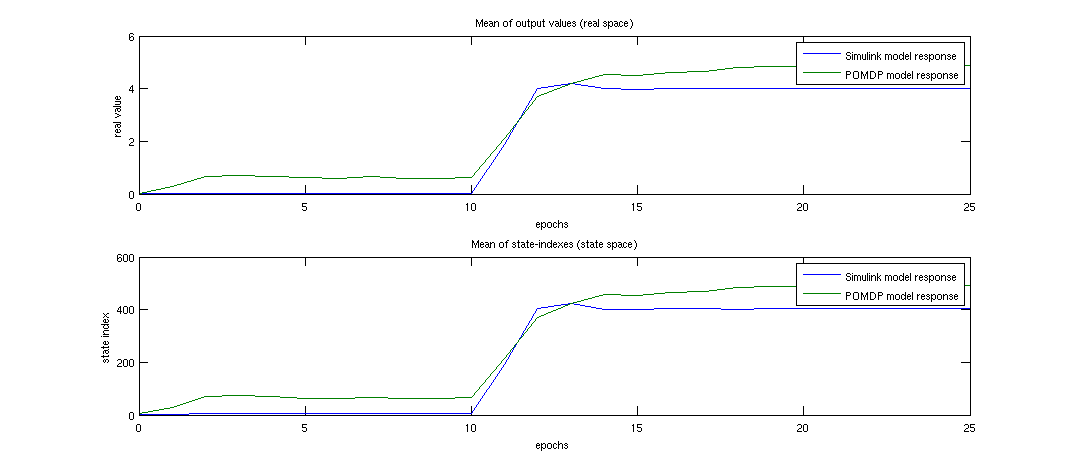
\includegraphics[width=18cm]{media/bw/bw_val_step_real_mean}\\
\end{center}
\caption{Plot of the real output value mean of Simulink and MDP responses to signal $u_2(t)$}
\label{bw_val_step_real_mean}
\end{figure}

The responses to the step input provide even more insight into the difference between the Simulink and the MDP system description. The next few paragraphs will again discuss the visible differences.

Similar as for the constant input signal, the discretization does not have a visible effect on the system responses. This can be seen by the lack of visible differences between the box plots of the Simulink responses in real and in state space as well as by looking at the differences between the response distributions of the MDP in the two spaces. In this case, the MDP also responds with a much stronger variance, indicating a less accurate system description. The responses do show, that both models react similarily and at the same time to the stimulation signal. Interestingly the MDP system settles at a slightly higher output value before and after the initial step. Interestingly these responses show an effect that was not noticable with the responses to the constant stimulation. The box plots show that the distribution variance only increases after the disturbance. The MDP's response variance before the step (at epoch 10) is suprisingly small. This may indicate a propagation effect, whereby the variance increases with every disturbance, as the resulting uncertainty propagates to later epochs.

Figure~\ref{bw_val_step_state_corr} shows the correlation between the responses' state space distributions for each epoch. The plot shows that the distributions do not correlate at all, except for epoch 13. The extremely low correlation will be discussed in more detail in chapter~\ref{discussion}, but is likely caused by initial state differences between the models. Similarily to the correlation in the previous section, the correlation also spikes just after the disturbance, indicating that, contrary to steady state, the models' reactions correlate strongly when the system is disturbed.

The plot of real and state output means in figure~\ref{bw_val_step_real_mean} show two interesting effects. Firstly the models seems to diverge even before the disturbance and secondly the systems diverge again after the disturbance. Yet, during the disturbance, the system react similarily. Although this causes for this are discussed in more detail in chapter~\ref{discussion}, this effect may, again, be caused by different inital states and the propagation of uncertainty after the disturbance.









